\documentclass[a4paper, 11pt]{report}
\usepackage[utf8]{inputenc}
\usepackage[T1]{fontenc}
\usepackage{lmodern}
\usepackage[french]{babel}
\usepackage{xcolor}
\usepackage{amssymb,amsmath}
\usepackage{fancyhdr}
\usepackage{ifxetex,ifluatex}
\usepackage{fixltx2e} % provides \textsubscript
% use upquote if available, for straight quotes in verbatim environments
\IfFileExists{upquote.sty}{\usepackage{upquote}}{}
\ifnum 0\ifxetex 1\fi\ifluatex 1\fi=0 % if pdftex
  \usepackage[utf8]{inputenc}
\else % if luatex or xelatex
  \ifxetex
    \usepackage{mathspec}
    \usepackage{xltxtra,xunicode}
  \else
    \usepackage{fontspec}
  \fi
  \defaultfontfeatures{Mapping=tex-text,Scale=MatchLowercase}
  \newcommand{\euro}{€}
\fi
% use microtype if available
\IfFileExists{microtype.sty}{\usepackage{microtype}}{}
\usepackage{graphicx}
% Redefine \includegraphics so that, unless explicit options are
% given, the image width will not exceed the width of the page.
% Images get their normal width if they fit onto the page, but
% are scaled down if they would overflow the margins.
\makeatletter
\def\ScaleIfNeeded{%
  \ifdim\Gin@nat@width>\linewidth
    \linewidth
  \else
    \Gin@nat@width
  \fi
}
\makeatother
\let\Oldincludegraphics\includegraphics
{%
 \catcode`\@=11\relax%
 \gdef\includegraphics{\@ifnextchar[{\Oldincludegraphics}{\Oldincludegraphics[width=\ScaleIfNeeded]}}%
}%
\ifxetex
  \usepackage[setpagesize=false, % page size defined by xetex
              unicode=false, % unicode breaks when used with xetex
              xetex]{hyperref}
\else
  \usepackage[unicode=true]{hyperref}
\fi
\hypersetup{breaklinks=true,
            pdfauthor={Thibault Deutsch (deutsc\_t); Rémy Bernier (bernie\_r); Marc Fresne (fresne\_m); Anthony Belthier (belthi\_a)},
            pdftitle={Cahiers des charges},
            colorlinks=true,
            citecolor=blue,
            urlcolor=blue,
            linkcolor=black,
            pdfborder={0 0 0}}
\urlstyle{same}  % don't use monospace font for urls
\setlength{\parindent}{0pt}
\setlength{\parskip}{6pt plus 2pt minus 1pt}
\setlength{\emergencystretch}{3em}  % prevent overfull lines
\setcounter{secnumdepth}{0}

\pagestyle{fancy}
\fancyhead[L]{Emagine Studio}
\fancyhead[C]{}
\fancyhead[R]{Troma}

\title{Cahier des charges}
\author{Thibault Deutsch (deutsc\_t) \and Rémy Bernier (bernie\_r) \and Marc Fresne (fresne\_m) \and Anthony Belthier (belthi\_a)}
\date{15 janvier 2014}

\begin{document}
\pagenumbering{Roman}

\thispagestyle{empty}
\begin{center}
{\fontsize{30}{32}{\textbf{Troma}}}
\par
\vspace*{0.5cm}
{\fontsize{20}{24}{{\textbf{Cahier des charges}}}}
\par
{\fontsize{15}{18}{{\textbf{\today}}}}
\end{center}

\vspace*{0.5cm}
\begin{figure}[htbp]
   \begin{center}
      
\includegraphics[scale = 0.05]{eie.png}
   \end{center}
\end{figure}

\vspace*{0.5cm}
\par
\begin{center}
\fontsize{16}{20}
\textbf{Thibault }
\emph{Dethi }
\textbf{Deutsch}
(\emph{deutsc\_t})
\newline
\textbf{Rémy }
\emph{Shadows }
\textbf{Bernier}
(\emph{bernie\_r})
\newline
\textbf{Marc }
\emph{Leshlague }
\textbf{Fresne}
(\emph{fresne\_m})
\newline
\textbf{Anthony }
\emph{AnthonySG }
\textbf{Belthier}
(\emph{belthi\_a})
\newline
\end{center}

\tableofcontents

\newpage
\textbf{{\huge Introduction}} \vspace{7mm}

Ce cahier des charges a pour but de présenter  le projet Troma, ainsi que l’équipe Emagine Studio chargée de sa réalisation.
Il explicite la nature du projet, les étapes nécessaires à son aboutissement mais aussi leur répartition par membre et dans le temps ainsi que les outils indispensables à sa réalisation.

Sa rédaction nous a permis d’organiser et de simplifier les différentes phases de développement en fixant des objectifs concrets à atteindre. Il représente la base de conception sur laquelle nous nous appuierons.
Il s’agit avant tout d’exposer les lignes directrices de notre projet et du planning de réalisation. De cette manière, après lecture, vous aurez donc pris connaissance des informations principales concernant le projet Troma qui vous sera présenté deux fois au court de son développement, puis une dernière fois dans sa version finale. \vspace{7mm}

\begin{figure}[htbp]
\centering

\includegraphics[scale=0.12]{troma.png}
\caption{Première version du logo de notre jeu}
\end{figure}

\newpage \section{Présentation des membres}\label{pruxe9sentation-des-membres}

\subsection{Thibault `Dethi' Deutsch \emph{(deutsc\_t)}}\label{thibault-dethi-deutsch-deutscux5ft}

Je suis passionné d'informatique depuis ma plus jeune enfance. J'ai une soif de savoir immense, ce qui me conduit à lire énormément et ainsi avoir des connaissances, dans de nombreux domaines, que je partage au maximum. La programmation est un de mes plus grands loisirs. Ce n'est pas mon premier projet. C'est pourquoi je partagerai mon expérience afin de mener à bien notre jeu jusqu'au bout ! Tout le défi pour moi résidera dans la programmation 3D. Pleins de nouvelles connaissances à venir !

\subsection{Rémy `Shadows' Bernier \emph{(bernie\_r)}}\label{ruxe9my-shadows-bernier-bernieux5fr}

Grand maigre métissé en classe de C2 venu de terminal S-Si. Je n'ai jamais codé avant EPITA et j'ai eu beaucoup de mal avec les langages de programmation, que ce soit CAML ou C\#. Me lancer dans un projet d'une telle ampleur me semblait insurmontable. Créer un jeu alors que l'on venait juste de commencer le C\# depuis 2 mois était impensable. Puis on acquière des facilitées grâce aux TPs et j'espère que ce projet m'apportera beaucoup de connaissance.

\subsection{Marc `Leshlague' Fresne \emph{(fresne\_m)}}\label{marc-leshlague-fresne-fresneux5fm}

J'ai toujours été intéressé par ce qui concerne l'informatique et l'électronique. C'est cet intérêt qui m'a conduit jusqu'à l'EPITA. Pourtant avant d'intégrer l'école je ne me suis pas plongé dans le C\# ou le CAML, à peine dans le C++ et l'HTML. Le projet de SUP me parait être une très bonne occasion d'approfondir les connaissances acquises pendant les cours et les TPs. La liberté accordée quant au type de programme qui nous est demandé de développer, va me permettre de réaliser une sorte de ''rêve'' commun a beaucoup de SUP : réaliser un jeu vidéo. Je suis donc comme les autres membres du groupe, c'est à dire super motivé pour mener à bien Troma, notre FPS.

\subsection{Anthony `AnthonySG' Belthier \emph{(belthi\_a)}}\label{anthony-anthonysg-belthier-belthiux5fa}

Je suis un jeune geek passionné de technologie et amateur de programmation. Je viens tout droit du 91 pour m'améliorer ! Je cherche toujours à produire le meilleur de moi-même et espère mener ce projet encore plus loin que loin (et oui).

\newpage
\section{Présentation du projet}\label{pruxe9sentation-du-projet}

\subsection{Type de projet}\label{type-de-projet}

Dès novembre, quand notre équipe fut complète, nous avons cherché une idée à réaliser. Dès le départ nous avons décidé de réaliser un jeu vidéo. L'idée était plus que motivante pour l'ensemble de l'équipe. De plus, nous avions toujours voulu connaître quels était les secrets de cette industrie.

On sait également, par expérience de l'un de nos membres, que le défi est intéressant. De nombreuses problématiques, de nombreux algorithmes à apprendre, etc. De plus un jeu vidéo implique une grande créativité. Nous sommes totalement libre au niveau des graphismes, du son, des fonctionnalités, etc.

Notre première idée de jeu vidéo était un Tower Defense version navale. Le jeu était en 2D et les graphismes auraient été entièrement réalisés par nous-même. Cependant nous étions bloqués sur le Game Design du jeu. Nous n'arrivions pas à créer un jeu qui tienne vraiment la route. Certaines fonctions rendaient le jeu injouable. Du coup, nous avons décidé de pousser le défi plus loin et de partir sur de la 3D. Ceci permettra également de nous démarquer des autres groupes.

A partir de ce moment là, notre idée de jeu était claire. Ce sera un First-Person shooter, abrégé dorénavant FPS, ou rien ! En effet, c'est le seul type de jeu que l'ensemble de l'équipe apprécie. Il nous restait alors à définir l'idée principale du jeu, son thème et son nom.

Nous avons choisi de réaliser un FPS dont le but est de tuer l'ensemble des cibles du parcours avec le meilleur temps possible. Ce type de niveau s'apparente un peu au mode d'entrainement que l'on peut retrouver dans les grands opus. Notre jeu comportera également un mode multijoueur, qui permettra à plusieurs joueurs de s'affronter en temps réel sur une carte. Le but étant alors d'obtenir le meilleur score, défini par le ratio entre le nombre de personnes tuées et de mort.

\subsection{Petite précision sur les FPS}\label{petite-pruxe9cision-sur-les-fps}

Le FPS désigne un certain type de jeu vidéo. En français, on dit qu'il s'agit d'un jeu de tir en vue subjective. C'est-à-dire un jeu de tir à la première personne. Cela implique que le joueur voit au travers du regard du personnage. Ce genre est apparu avec les jeux Maze War et Spasim sortis en 1974 mais a été popularisé par Doom en 1993 ! Aujourd'hui c'est un des types de jeu les plus vendus au monde, on pourra citer comme exemple la série des Call of Duty ou encore celle des Battlefield.

\begin{figure}[htbp]
\centering
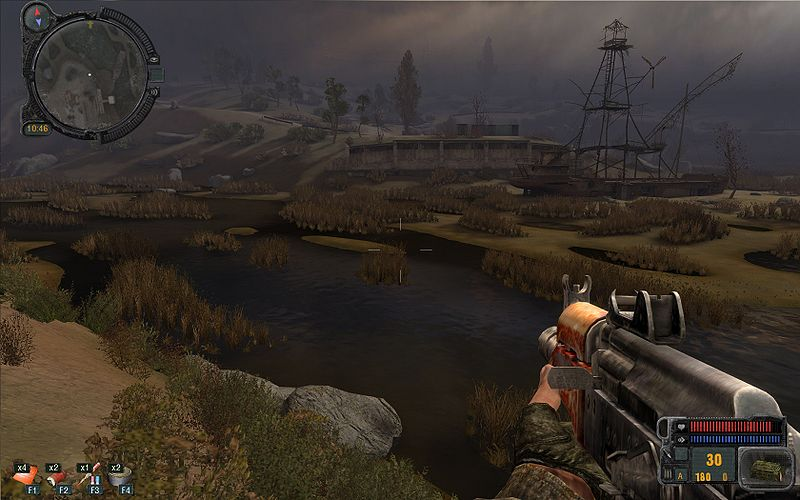
\includegraphics[scale=0.4]{exemple_FPS.jpg}
\caption{Capture d'écran de S.T.A.L.K.E.R.: Call of Pripyat (2009)}
\end{figure}

\subsection{Thème et nom du projet}\label{thuxe8mes-et-noms-du-projet}

Pour le thème, nous avons choisi la seconde guerre mondiale. Ceci nous permettra de nous distinguer des récents grands opus, qui ont tous décidés de se concentrer sur le monde actuel ou le futur. Créer un jeu sur la seconde guerre mondiale implique également un minimum de recherche pour pouvoir respecter le contexte historique et donc rendre le jeu réaliste. Ainsi nous aurons un point de départ solide.

Une fois la conception de notre idée fini, nous avons mené un brainstorming sur les noms possibles. Au début nous n'avions que des noms hors contexte. Rien de très intéressant. Rien qui n'attire l'attention. Puis, par chance ou par hasard total, la télévision nous a donné la réponse. Aux informations, un reportage sur les spectacles de Dieudonné. Il nous est alors apparu le mot traumatisme. Cette guerre a été et est encore un grand traumatisme pour le monde entier. Une guerre sanglante. Mais le mot traumatisme est trop long. Alors nous avons poussé notre réflexion jusqu'à trauma.

\begin{quote}
``Un trauma est une blessure physique ou psychique infligée à l'organisme, ou la lésion locale qui en résulte. Le traumatisme renvoie quant à lui aux conséquences locales ou générales du trauma.'', \emph{Wikipédia}
\end{quote}

Comme le montre cette définition, les deux mots sont intimement liés. Mais nous sommes allés encore plus loin. Nous avons décidé de surpasser l'orthographe du mot. Ainsi notre jeu s'appelle Troma. Court, évoquant, surprenant et, même si vous ne le voulez pas, il est déjà incrusté dans votre esprit !

\newpage
\section{Buts et intérêts du projet}\label{buts-et-intuxe9ruxeats-du-projet}

Dans un premier temps ce projet va nous permettre d'apprendre à travailler en groupe. Il est primordial, sur un projet de cette envergure (plusieurs mois) de savoir répartir les tâches et déléguer aux différents membres du groupe. C'est ce sur quoi nous nous sommes penché en premier lieu afin de pouvoir immédiatement essayer d'optimiser notre temps. La deuxième étape a été d'apprendre à écouter et comprendre les autres. Nous pouvons avoir des avis différents sur un même sujet et il est important de savoir en tirer profit pour enrichir notre projet plutôt que l'inverse! Il est aussi question de travailler en suivant ``l'idée'' de quelqu'un d'autre. Certains s'y connaissant mieux dans certains domaines que d'autres, et inversement le fait de pouvoir suivre quelqu'un, va nous permettre de partager nos connaissances et d'avancer plus rapidement sur notre projet. Enfin il me semble extrêmement important de rester solidaire et de soutenir les autres membres du projet tout au long de celui-ci. Nous sommes avant tout une équipe et nous avons envie de faire du mieux que nous pouvons et donc de travailler tous ensemble !

Un autre intérêt de ce projet est l'apprentissage de la gestion du temps, des contraintes, ainsi que des éventuels problèmes pouvant survenir à tous moments. Dans la mesure où chacun d'entre nous souhaite bien-évidemment poursuivre ses études et devenir ingénieur en informatique. Il me semble être plus qu'important d'être confronté dès aujourd'hui aux problèmes que nous rencontrerons dans note vie professionnelle. Ainsi savoir gérer toutes sortes de contraintes demeure l'un des intérêts clé de ce projet pour nous !

Durant la répartition des taches, un des buts de ce projet nous a également sauté aux yeux : savoir évaluer la quantité de travail, d'heures que représente une tâche. Il est beaucoup plus dur qu'il n'y paraît de savoir combien de temps nous prendra une tâche, alors que dans certains cas, nous ne savons même pas encore comment exactement l'accomplir !

Plus personnellement ce projet va nous permettre d'acquérir des connaissances aussi bien en matière de programmation et donc en C\#, qu'en termes de graphismes ou développement 3D. Une nouvelle fois cela représente un pas en avant vers le monde professionnel auquel nous serons confrontés. C'est pour cela que nous souhaitons au maximum que chacun d'entre nous comprenne l'ensemble des algorithmes ou ``procédés'' utilisés par les autres, pour mener à bien ce projet.

\newpage
\section{Budget}\label{budget}

Pour notre projet, nous aurons besoin de deux manettes Xbox 360, afin de pouvoir développer le jeu pour que celui-ci puisse interagir avec les manettes.

De plus pour la présence en ligne d'Emagine Studio, nous avons du acheter un nom de domaine et un mini serveur pour l'héberger. Le serveur pourra également nous servir pour le mode multijoueur de notre jeu.

Enfin, nous travaillerons principalement sur nos racks ou sur du matériel que nous avons déjà à notre disposition. Ces derniers ne rentrent donc pas dans le coût du projet.
\newline

\begin{figure}[htbp]
\centering
\begin{tabular}{ | l | l | }
\hline \textbf{Matériels, logiciels et services} & \textbf{Coût} \\
\hline Racks & 80€/personne \\
\hline Manette Xbox 360 & 40€ \\
\hline Visual Studio & Offert par EPITA \\
\hline Audacity & Gratuit \\
\hline Blender & Gratuit \\
\hline The GIMP & Gratuit \\
\hline Mini VPS & 5€/mois \\
\hline Nom de domaine & 8€/an \\
\hline Main d'oeuvre & Bénévolat \\
\hline Heure de sommeil perdu & Non rattrapable, donc 10€/h \\
\hline \textbf{Total} & 1868€ \\
\hline 
\end{tabular}
\end{figure}

\newpage
\section{Les différents logiciels utilisés}\label{les-diffuxe9rents-logiciels-utilisuxe9s}

\subsection{XNA}\label{xna}

XNA est un moteur graphique qui devra gérer l'environnement, les déplacements, la caméra, les objets 3D et les animations. Nous souhaiterions aussi créer des interactions entre l'environnement et le moteur Graphique (inclinaison automatique de la caméra en fonction de la position du curseur de la souris par exemple).

\subsection{Audacity}\label{audacity}

Audacity est un logiciel de montage audio qui nous permettra de créer des sons à partir de notre propre voix ou de son pris sur internet (bruitages, coup de feu d'une arme, explosion\ldots{}). Il n'y a rien de pire qu'un jeu sans son pour un joueur. On a choisi ce logiciel car il est gratuit.

\subsection{Blender}\label{blender}

Blender est un logiciel de modélisation 3D qui nous servira à créer le décor du jeu (tous ce qui est mur, objet sur la carte) et aussi les personnages et les armes. On a choisi Blender car c'est un logiciel gratuit et performant.

\subsection{\LaTeX}\label{latex}

\LaTeX est un système de mise en page qui nous a permit de créer notre cahier des charges et notre rendu de chaque soutenance. Nous avons choisi \LaTeX car on y était obligé, ceci étant, c'est un très bon logiciel qui nous permet de faire de très beau dossier.

\subsection{Bitbucket}\label{bitbucket}

Bitbucket est un service de gestion de versions décentralisé. Il permet de mettre notre code en ligne pour toutes les personnes faisant partie du groupe. On peut donc regarder ce que les autres ont fait, leurs avancements, si on corrige une partie de code, celle-ci sera envoyée en ligne avec la modification. Nous l'avons choisi parce que pour les étudiants, le site nous donne un droit de dépôts privés illimités.

\newpage
\section{Découpage du projet}\label{duxe9coupage-du-projet}

\subsection{Modélisation}\label{moduxe9lisation}

Cette partie regroupe tout ce qui concerne la création du monde dans lequel le joueur évoluera plus tard, c'est-à-dire la création des cartes, la modélisation 3D du personnage, des armes et de divers autres objets. Il faut ajouter à tout ça la création de texture.

\subsection{Moteur graphique}\label{moteur-graphique}

Pour le moteur graphique nous utiliserons XNA 4. Il aura la tâche d'afficher les diverses textures et modèles de manière suffisamment fluide.

\subsection{Moteur physique}\label{moteur-physique}

Le moteur physique devra gérer les nombreuses collisions. De plus il devra également fournir un moteur de particule afin de pouvoir donner l'illusion d'explosion.

\subsection{Menu}\label{menu}

Le menu regroupera différents écrans, tel que l'écran de démarrage, l'écran en partie ou encore l'écran de fin de partie. Il devra également permettre au joueur de choisir entre les différents modes de jeu. Des options seront présentes dans le menu pour permettre au joueur de changer différents réglages.

\subsection{Réseau}\label{ruxe9seau}

Un FPS est en général bien plus attractif en multijoueur. C'est pourquoi nous implémenterons un mode multijoueur en réseau. Un serveur servira de point de relai entre tous les joueurs de la partie pour synchroniser les informations en temps réel entre eux.

\subsection{Gameplay}\label{gameplay}

Le gameplay regroupe le contrôle du personnage, la gestion des armes et des points de vie. Le score appartient également au gameplay et c'est celui-ci qui rendra le jeu attractif pour le joueur.

\subsection{Audio}\label{audio}

L'audio est un élément essentiel dans un jeu. Pour cela nous devrons gérer de multiples bruitages en même temps.

\subsection{Site web}\label{site-web}

Le site web présentera notre projet. Il comportera diverses pages de présentation ainsi qu'un blog pour tenir informé sur le développement de notre jeu. De plus nous devrons marquer notre présence sur les réseaux sociaux.

\newpage
\section{Répartition des tâches}\label{repartition-des-tuxe2ches}
\colorlet{darkgreen}{green!60!black}

\subsection{Première soutenance}\label{premiuxe8re-soutenance}

\begin{tabular}{ | c || c | c | c | c | }
\hline Tâches & Thibault & Rémy & Marc & Anthony \\
\hline Modélisation & & & \textcolor{orange}{X} & \textcolor{orange}{X} \\
\hline Moteur graphique & \textcolor{red}{X} & & \textcolor{red}{X} & \\
\hline Moteur physique & & \textcolor{red}{X} & & \textcolor{red}{X} \\
\hline Menu & & \textcolor{red}{X} & & \textcolor{red}{X} \\
\hline Réseau & & & & \\
\hline Gameplay & \textcolor{orange}{X} & \textcolor{orange}{X} & \textcolor{orange}{X} & \\
\hline Audio & & \textcolor{red}{X} & & \textcolor{red}{X} \\
\hline Site web & \textcolor{orange}{X} & \textcolor{orange}{X} & & \\
\hline
\end{tabular}

\subsection{Deuxième soutenance}\label{deuxiuxe8me-soutenance}

\begin{tabular}{ | c || c | c | c | c | }
\hline Tâches & Thibault & Rémy & Marc & Anthony \\
\hline Modélisation & & & \textcolor{orange}{X} & \textcolor{orange}{X} \\
\hline Moteur graphique & \textcolor{orange}{X} & & \textcolor{orange}{X} & \\
\hline Moteur physique & & \textcolor{orange}{X} & & \textcolor{orange}{X} \\
\hline Menu & & \textcolor{orange}{X} & & \textcolor{orange}{X} \\
\hline Réseau & \textcolor{red}{X} & & \textcolor{red}{X} & \textcolor{red}{X} \\
\hline Gameplay & \textcolor{orange}{X} & \textcolor{orange}{X} & & \\
\hline Audio & & \textcolor{darkgreen}{X} & & \textcolor{darkgreen}{X} \\
\hline Site web & \textcolor{darkgreen}{X} & \textcolor{darkgreen}{X} & & \\
\hline
\end{tabular}

\subsection{Soutenance finale}\label{soutenance-finale}

\begin{tabular}{ | c || c | c | c | c | }
\hline Tâches & Thibault & Rémy & Marc & Anthony \\
\hline Modélisation & & & \textcolor{darkgreen}{X} & \textcolor{darkgreen}{X} \\
\hline Moteur graphique & \textcolor{darkgreen}{X} & & \textcolor{darkgreen}{X} & \\
\hline Moteur physique & & \textcolor{darkgreen}{X} & & \textcolor{darkgreen}{X} \\
\hline Menu & & \textcolor{darkgreen}{X} & & \textcolor{darkgreen}{X} \\
\hline Réseau & \textcolor{darkgreen}{X} & & \textcolor{darkgreen}{X} & \textcolor{darkgreen}{X} \\
\hline Gameplay & \textcolor{darkgreen}{X} & \textcolor{darkgreen}{X} & & \\
\hline Audio & & \textcolor{darkgreen}{X} & & \textcolor{darkgreen}{X} \\
\hline Site web & \textcolor{darkgreen}{X} & \textcolor{darkgreen}{X} & & \\
\hline
\end{tabular}

\vspace*{7mm}
\textbf{Légende :}
\begin{itemize}
  \item \textcolor{red}{Rouge} : Commencé
  \item \textcolor{orange}{Orange} : Avancé
  \item \textcolor{darkgreen}{Vert} : Terminé
\end{itemize}

\newpage
\textbf{{\huge Conclusion}} \vspace{7mm}

Nous avons présenté l’ensemble des points à abordés, ainsi s’achève notre cahier des charges.
Nous espérons respecter le planning que nous nous sommes fixés, aussi bien au niveau du contenu qu’au niveau des dates. Nous espérons que nous aurons le temps d’ajouter d’autres fonctionnalités ainsi qu’améliorer le plus possible la qualité graphique du jeu.

Nous sommes confiants quant à ces objectifs puisque nous sommes très motivés par l’idée d’avoir réussi à concevoir notre jeu, mais aussi car il s’agit d’une occasion à ne pas rater pour réaliser un projet en équipe et approfondir nos connaissances dans divers domaines. Tout ceci annonce de bonne soirée !

\end{document}